\documentclass[pdf]{beamer}
\mode<presentation>{} 

\usepackage{hyperref}
\usepackage{pgf}
\usepackage{fancyhdr}
\usepackage{tikz}
\usetikzlibrary{trees}
\usetikzlibrary{arrows,automata}
\usetikzlibrary{automata,positioning}
\usetikzlibrary{shapes}
\usepackage{tikz-qtree,tikz-qtree-compat}
\usepackage{mathtools,enumerate,amssymb}
\usetikzlibrary{patterns}
\usepackage[utf8]{inputenc}
\usepackage[T1]{fontenc}
\usepackage{graphicx}
\usepackage{varwidth}
\usepackage{xcolor}
\usepackage{multicol}
\usepackage{multirow}
\usepackage[export]{adjustbox}
%\usepackage{subfig}
\usepackage{wrapfig}
\usepackage{textcomp}
\usepackage{eso-pic}
\usepackage{pgfornament}
\usepackage[export]{adjustbox}



\newcommand\PlaceText[3]{%
\begin{tikzpicture}[remember picture,overlay]
\node[outer sep=0pt,inner sep=0pt,anchor=south west] 
  at ([xshift=#1,yshift=-#2]current page.north west) {#3};
\end{tikzpicture}%
}



\definecolor{Blue}{RGB}{0,0,100}
\definecolor{background}{RGB}{255,255,255}


\title{Design of everyday things}
\subtitle{Human Computer Interaction}
\AtBeginSection[]{}



\setbeamertemplate{sidebar right}{}
\setbeamertemplate{footline}{%
\hfill\usebeamertemplate***{navigation symbols}
\hspace{1cm}\insertframenumber{}/\inserttotalframenumber}

\graphicspath{{./img/}}



\begin{document}



{\setbeamercolor{background canvas}{bg=background}
\begin{frame}
\vspace{10mm}
\huge{\raggedleft{\color{black}{\textbf{Design of everyday things}}}}

\large{\raggedleft{\color{black} Human Computer Interaction}}

\begin{flushright}
\end{flushright}

\fontsize{7pt}{1pt}\selectfont{
Based on slide deck 

\textbf{Part 4: Designing and building visual interfaces. Design of everyday things}

Human Computer Interaction I: Principles and Design

by

\textbf{Saul Greenberg}
\newline
Professor
\newline
\textbf{University of Calgary, Canada}

\textit{The new slides are marked with a *}
}

\fontsize{5pt}{1pt}\selectfont{ \textcolor{lightgray}
{Slide deck by Saul Greenberg. Permission is granted to use this for non-commercial purposes as long as general credit to Saul Greenberg is clearly maintained.
Warning: some material in this deck is used from other sources without permission. Credit to the original source is given if it is known.}}

\end{frame}}



% Inaintea codului fiecarui slide se vor scrie urmatoarele informatii:
% Nume si prenume student
% Numarul slide-ului corespunzator din prezentarea prof. Saul Greenberg
% Numele imaginilor inserate trebuie sa fie numar_slide_nume_imagine.extensie_imagine



% Nitica Razvan Alexandru
% Numarul slide-ului: 1
\begin{frame}
	{Design of everyday things}{\textcolor{red}{\rule{12cm}{1.2pt}}}
	\textbf{Summary so far}
	
    \begin{itemize}
      \item [--]many so-called human errors are actually errors in design
      \item [--]human factors became important as human performance limitations reached when handling complex machinery
    \end{itemize}
\end{frame}



\begin{frame}
	{Design of everyday things}{\textcolor{red}{\rule{12cm}{1.2pt}}}

    \textbf{Important concepts for designing everyday things}
    
    \begin{itemize}
      \item [--]perceived affordances
      \item [--]causality
      \item [--]visible constraints
      \item [--]mapping
      \item [--]transfer effects
      \item [--]idioms \& population stereotypes
      \item [--]cultural associations
      \item [--]conceptual models
      \item [--]individual differences
      \item [--]why design is hard
    \end{itemize}
\end{frame}



% Nitica Razvan Alexandru
% Numarul slide-ului: 2

\begin{frame}
{Perceived Affordances}{\textcolor{red}{\rule{12cm}{1.2pt}}}

\textbf{The perceived properties of the object that suggest how one could use it}

\begin{figure}
\centering
chairs are for sitting, table for placing things on
\includegraphics[width=0.4\textwidth]{2_chairs.png}

knobs are for turning
\newline
\includegraphics[width=0.4\textwidth]{2_knobs.jpg}
%  \vfill
%  \subfloat[slots are for inserting handles are for turning]{\includegraphics[width=0.3\textwidth]{2_slots.jpg}}
%  \vspace{2cm}
%  \subfloat[buttons are for pressing]{\includegraphics[width=0.2\textwidth]{2_buttons.jpg}}
%  \vspace{2cm}
%  \subfloat[switch for toggling]{\includegraphics[width=0.15\textwidth]{2_switch.png}}
%  \vspace{2cm}
%  \subfloat[computer for…]{\includegraphics[width=0.2\textwidth]{2_computer.jpg}}
%  \vspace{2cm}
\end{figure}
\end{frame}



\begin{frame}
{Perceived Affordances}{\textcolor{red}{\rule{12cm}{1.2pt}}}

\begin{figure}
\centering

slots are for inserting, handles are for turning
\newline
\includegraphics[width=0.3\textwidth]{2_slots.jpg}

buttons are for pressing
\newline
\includegraphics[width=0.2\textwidth]{2_buttons.jpg}

\end{figure}
\end{frame}



\begin{frame}
{Perceived Affordances}{\textcolor{red}{\rule{12cm}{1.2pt}}}

\begin{figure}
\centering

switch for toggling
\newline
\includegraphics[width=0.15\textwidth]{2_switch.png}

computer for ... ?
\newline
\includegraphics[width=0.2\textwidth]{2_computer.jpg}

\end{figure}
\end{frame}



% Nitica Razvan Alexandru
% Numarul slide-ului: 3

\begin{frame}
{Perceived Affordances}{\textcolor{red}{\rule{12cm}{1.2pt}}}
\textbf{Product design}
\begin{itemize}
	\item [--]perceived affordances:
		\begin{itemize}
			\item[\textcolor{black}{•}]design invites people to take possible actions
		\end{itemize}
	\item[--]actual affordances: 
		\begin{itemize}
			\item[\textcolor{black}{•}]the actual actionable properties \newline of the product
		\end{itemize}
	\end{itemize}
\bigskip \bigskip \bigskip \bigskip \bigskip \bigskip
\textbf{Problems occur when}
\begin{itemize}
	\item[--]these are not the same
	\item[--]people's perceptions are not what the \newline designer expects
\end{itemize}
\begin{picture}(0,0)
      \put(200,0){\hbox{\includegraphics[scale=0.4]{3_picture.jpg}}}
  	\end{picture}
\end{frame}



% Nitica Razvan Alexandru
% Numarul slide-ului: 4

\begin{frame}
{Perceived Affordances}{\textcolor{red}{\rule{12cm}{1.2pt}}}
\begin{picture}(0,0)
	\put(-25,-130){\hbox{\includegraphics[scale=0.7]{4_picture.PNG}}}
\end{picture}
\end{frame}



% Nitica Razvan Alexandru
% Numarul slide-ului: 5

\begin{frame}
{Perceived Affordance Problems}{\textcolor{red}{\rule{12cm}{1.2pt}}}
\begin{picture}(0,0)
	\put(-25,-130){\hbox{\includegraphics[scale=0.7]{5_picture.PNG}}}
\end{picture}
\end{frame}



% Nitica Razvan Alexandru
% Numarul slide-ului: 6

\begin{frame}
{Perceived Affordances}{\textcolor{red}{\rule{12cm}{1.2pt}}}
\textbf{GUI design}
\begin{itemize}
	\item [--]perception only through visuals
	\item [--]designer creates appropriate visual affordances via
	\begin{itemize}
		\item [\textcolor{black}{•}]familiar idioms
        \item [\textcolor{black}{•}]metaphors
	\end{itemize}
\end{itemize}
\bigskip \bigskip \bigskip \bigskip \bigskip \bigskip \bigskip \bigskip \bigskip \bigskip \bigskip
\begin{picture}(0,0)
      \put(130,0){\hbox{\includegraphics[scale=0.5]{6_picture.png}}}
  	\end{picture}
\end{frame}



% Nitica Razvan Alexandru
% Numarul slide-ului: 7

\begin{frame}
{Perceived Affordances}{\textcolor{red}{\rule{12cm}{1.2pt}}}
\begin{picture}(0,0)
      \put(-20,-120){\hbox{\includegraphics[scale=0.7]{7_picture.PNG}}}
  	\end{picture}
\end{frame}



% Nitica Razvan Alexandru
% Numarul slide-ului: 8

\begin{frame}
{Perceived Affordance Problems}{\textcolor{red}{\rule{12cm}{1.2pt}}}
\begin{picture}(0,0)
      \put(-27,-120){\hbox{\includegraphics[scale=0.7]{8_picture.PNG}}}
  	\end{picture}
\end{frame}



% Oprea Edward-Cosmin
% Numarul slide-ului :9

\begin{frame}
{Perceived Affordance Problems}{\textcolor{red}{\rule{12cm}{1.2pt}}}
\begin{picture}(0,0)
	\put(-27,-120){\hbox{\includegraphics[scale=0.7]{9_IBMtelephone.PNG}}}
\end{picture}
\end{frame}



% Oprea Edward-Cosmin
% Numarul slide-ului :10

\begin{frame}
{Perceived Affordance Problems}{\textcolor{red}{\rule{12cm}{1.2pt}}}
\begin{picture}(0,0)
	\put(50,-100){\hbox{\includegraphics[scale=0.5]{10_IBMtelephone.png}}}
\end{picture}
\end{frame}



% Oprea Edward-Cosmin
% Numarul slide-ului :11

\begin{frame}
{Perceived Affordance Problems}{\textcolor{red}{\rule{12cm}{1.2pt}}}
Handles are for lifting,
\newline but these are for scroling!
\begin{picture}(0,0)
	\put(-120,-85){\hbox{\includegraphics[scale=0.5]{11_equalizer.PNG}}}
\end{picture}
\newline \newline \newline
\newline \newline \newline
\newline 
Complex things may need explaining but
\newline simple things should not
\begin{itemize}
      \item [--]when simple things need labels \& instructions, then design has failed
 \end{itemize}
\end{frame}



% Oprea Edward-Cosmin
% Numarul slide-ului :12

\begin{frame}
{Visible Constraints}{\textcolor{red}{\rule{12cm}{1.2pt}}}
Limitations of actions possible perceived from object's appearance
 \begin{itemize}
      \item [--]provides people with a range of ussage possibilites
 \end{itemize}
 \begin{picture}(0,0)
	\put(50,-120){\hbox{\includegraphics[scale=0.55]{12_limitations.PNG}}}
\end{picture}
\newline \newline \newline
\newline \newline \newline
\newline \newline \newline

\end{frame}



% Oprea Edward-Cosmin
% Numarul slide-ului :13

\begin{frame}
{Visible Constraints Problems}{\textcolor{red}{\rule{12cm}{1.2pt}}}

Which side do you use for cutting?

\begin{figure}
	\includegraphics[scale=0.50]{13_knife.png}
\end{figure}
\end{frame}



% Oprea Edward-Cosmin
% Numarul slide-ului :14

\begin{frame}
{Visible Constraints:Entering a Date}{\textcolor{red}{\rule{12cm}{1.2pt}}}
The more constraints, the less opportunity for error
 \begin{itemize}
      \item [--]particularly important for managing user input
 \end{itemize}
 \begin{picture}(0,0)
	\put(10,-130){\hbox{\includegraphics[scale=0.45]{14_form1.png}}}
\end{picture} 
 \begin{picture}(0,0)
	\put(140,-130){\hbox{\includegraphics[scale=0.45]{14_form2.png}}}
\end{picture} 
\newline \newline \newline
\newline \newline \newline
\newline \newline \newline
 
\end{frame}



% Oprea Edward-Cosmin
% Numarul slide-ului :16

\begin{frame}{Visible Constraints Problems}{\textcolor{red}{\rule{12cm}{1.2pt}}}

\begin{figure}[b]
    	\includegraphics[scale = 0.40, center]{16_cooker.jpg}
    \end{figure}
\end{frame}



% Paun Razvan Gabriel
% Numarul slide-ului: 17

\newlength{\seplinewidth}
\newlength{\seplinesep}
\setlength{\seplinewidth}{1mm}
\setlength{\seplinesep}{2mm}
\colorlet{sepline}{red}
\newcommand*{\sepline}{%
  \par
  %\vspace{\dimexpr\seplinesep+.5\parskip}%
  \cleaders\vbox{%
    \begingroup % because of color
      \color{sepline}%
      \hrule width\linewidth height\seplinewidth
    \endgroup
  }\vskip\seplinewidth
  \vspace{-0.85cm}
  %\vspace{\dimexpr\seplinesep-.5\parskip}%
}
\begin{frame}{Mapping}{\textcolor{red}{\rule{12cm}{1.2pt}}}

\begin{figure}[b]
    	\includegraphics[scale = 0.19, center]{17_Picture.jpg}
    \end{figure}

\end{frame}



% Paun Razvan Gabriel
% Numarul slide-ului: 18

\begin{frame}
    {Mapping}{\textcolor{red}{\rule{12cm}{1.2pt}}}
    
    The set of possible relations between objects \par
    Control-display compatibility \par \par
    \begin{itemize}
    \item[\textcolor{black}{--}] the natural relationship between controls and displays
      \item[\textcolor{black}{--}] e.g., visual mapping of stove controls to elements
     

    \end{itemize}
    
    \begin{figure}[b]
    	\includegraphics[scale = 0.69, center]{18_Picture.png}
    \end{figure}
  
\end{frame}



% Paun Razvan Gabriel
% Numarul slide-ului: 19

\begin{frame}
    {Mapping}{\textcolor{red}{\rule{12cm}{1.2pt}}}
    
 	Control-display compatibility
    \begin{itemize}    
    \item[\textcolor{black}{--}] mimic diagrams for feedback / control imitates physical layout
 
    \end{itemize}
    
    \begin{figure}[b]
    	\includegraphics[scale = 0.5, center]{19_Picture.jpg}
    \end{figure}
\end{frame}



% Paun Razvan Gabriel
% Numarul slide-ului: 20

\begin{frame}
    {Mapping}{\textcolor{red}{\rule{12cm}{1.2pt}}}
    
 	Control-display compatibility
    \begin{itemize}    
    \item[\textcolor{black}{--}] cause and effect 
 	\end{itemize}
 	\bigskip \bigskip \bigskip \bigskip \bigskip \bigskip
    \bigskip \bigskip \bigskip \bigskip \bigskip \bigskip
    
 	  \begin{picture}(0,0)
    \put(0,-10){\hbox{\includegraphics[scale=0.7]{20_Picture1.PNG}}}
    \end{picture}
    
    
      \begin{picture}(0,0)
    \put(140,5){\hbox{\includegraphics[scale=0.7]{20_Picture2.PNG}}}
    \end{picture}
    
    \begin{multicols}{2}
    steering wheel-turn left,\linebreak car turns left \linebreak
	scroll bar – scroll \linebreak down, viewport goes down
    \end{multicols}
\end{frame}



% Paun Razvan Gabriel
% Numarul slide-ului: 21

\begin{frame}
    {Mapping}{\textcolor{red}{\rule{12cm}{1.2pt}}}
    
   \Large Palette controls and active objects \normalsize
   \newline \linebreak 
   
    \begin{picture}(0,0)
    \put(0,-140){\hbox{\includegraphics[scale=0.63,right]{21_Picture.PNG}}}
    \end{picture} \small
   	Only controls that can
    \newline operate on a picture are
    \newline fully visible
    \linebreak \linebreak \linebreak
	Others are grayed out
    \linebreak \linebreak \linebreak \linebreak 
 	Selected picture
\end{frame}



% Paun Razvan Gabriel
% Numarul slide-ului: 22

\begin{frame}
    {Mapping}{\textcolor{red}{\rule{12cm}{1.2pt}}}
    
   \Large Action feedback \normalsize

   \begin{flushright}\footnotesize
   Cursor re-enforces
   \par selection of current item
   \par ...\linebreak \linebreak \linebreak \linebreak \linebreak \linebreak
   \end{flushright}
	\footnotesize
   Depressed button \par indicates current \par mapped item
   
   \begin{picture}(0,10)
    \put(0,0){\hbox{\includegraphics[scale=0.7,right]{22_Picture.PNG}}}
    \end{picture}
  
\end{frame}



% Paun Razvan Gabriel
% Numarul slide-ului: 23

\begin{frame}
    {Mapping Problems}{\textcolor{red}{\rule{12cm}{1.2pt}}}
    
   \Large Quick, open the top drawer \normalsize
   \linebreak \linebreak \linebreak \linebreak
   \newline \newline \newline \newline 
    \bigskip \bigskip \bigskip
     \bigskip \bigskip \bigskip \bigskip \bigskip \bigskip
   \begin{picture}(0,0)
    \put(-175,-93){\hbox{\includegraphics[scale=0.53,right]{23_Picture1.jpg}}}
    \end{picture}
    
    \begin{picture}(0,0)
    \put(15,20){\hbox{\includegraphics[scale=0.53,right]{23_Picture2.png}}}
    \end{picture}
  
\end{frame}



% Paun Razvan Gabriel
% Numarul slide-ului: 24

\begin{frame}
    {Mapping Problems}{\textcolor{red}{\rule{12cm}{1.2pt}}}
    
   \large Where do you plug in the mouse? \normalsize
   
   \begin{flushright}\small
   Mapping\par
   ambiguous
   \end{flushright}
   
   
     \bigskip \bigskip \bigskip
     \bigskip \bigskip \bigskip \bigskip \bigskip \bigskip\bigskip \bigskip \bigskip
     \bigskip \bigskip \bigskip \bigskip \bigskip \bigskip\bigskip \bigskip \bigskip
     \bigskip \bigskip \bigskip \bigskip \bigskip \bigskip
     \begin{picture}(0,0)
    \put(-55,54){\hbox{\includegraphics[scale=0.6,right]{24_Picture.jpg}}}
    \end{picture}
\end{frame}



% Popa Andrei Marius
% Numarul slide-ului: 25

\begin{frame}
{Causality}{\textcolor{red}{\rule{12cm}{1.2pt}}}

the thing that happens right after an action is assumed by people to be caused by that action
 \begin{itemize}
      \item [--]interpretation of "feedback"
 \end{itemize}
 \begin{itemize}
      \item [--]false causality
      \begin{itemize}
     		\item[\textcolor{black}{•}]incorrect effect
         		\begin{itemize}
         			\item [--]invoking unfamiliar function just as computer hangs
				\end{itemize}
                \begin{itemize}
                	\item [--]causes "superstitious" behaviours
                \end{itemize}
      		\end{itemize}
      \begin{itemize}
      		\item[\textcolor{black}{•}]invisible effect
         		\begin{itemize}
         			\item [--]command with no apparent result often re-entered repeatedly
				\end{itemize}
                \begin{itemize}
                	\item [--]e.g., mouse click to raise menu on unresponsive system
		        \end{itemize}
 	 \end{itemize}
\end{itemize}
\end{frame}



% Popa Andrei Marius
% Numarul slide-ului: 26

\begin{frame}
{Causality Problems}{\textcolor{red}{\rule{12cm}{1.2pt}}}
Effects visible only after Exec button is pressed
\begin{itemize}
	\item [--]Ok does nothing!
\end{itemize}
\begin{itemize}
	\item [--]awkward to find appropriate color level
\end{itemize}
\bigskip \bigskip \bigskip \bigskip \bigskip \bigskip
    \bigskip \bigskip \bigskip
\begin{picture}(0,0)
    \put(20,0){\hbox{\includegraphics[scale=0.50,left]{26_1.png}}}
    \end{picture} \small
     \begin{picture}(1,0)
    
    \begin{picture}(0,1)
    \put(-20,0){\hbox{\includegraphics[scale=0.50,right]{26_2.png}}}
    \end{picture} \small
    \begin{picture}(1,0)
    \put(20,-15){\hbox{\includegraphics[scale=0.50,left]{26_3.png}}}
    \end{picture} \small
    \put(-60,5){\hbox{\includegraphics[scale=0.50,right]{26_4.png}}}
    \end{picture} \small
\end{frame}



% Popa Andrei Marius
% Numarul slide-ului: 27

\begin{frame}
{Transfer Effects}{\textcolor{red}{\rule{12cm}{1.2pt}}}
People transfer their learning/expectations of similar objects to the current objects
\begin{itemize}
	\item[\textcolor{black}{•}]positive transfer: previous learnings also apply to new situation
\end{itemize}
\begin{itemize}
	\item[\textcolor{black}{•}]negative transfer: previous learnings conflict with the new situation
\end{itemize}
\bigskip \bigskip \bigskip \bigskip \bigskip \bigskip
\begin{picture}(0,0)
    \put(20,-10){\hbox{\includegraphics[scale=0.45,left]{27_1.png}}}
    \end{picture} \small
    \begin{picture}(0,1)
    \put(-120,30){\hbox{\includegraphics[scale=0.40,right]{27_2.png}}}
    \end{picture} \small
    \begin{picture}(1,0)
    \put(20,-15){\hbox{\includegraphics[scale=0.45,right]{27_3.png}}}
    \end{picture} \small
\end{frame}



% Popa Andrei Marius
% Numarul slide-ului: 29

\begin{frame}
{Transfer Effect Problems}{\textcolor{red}{\rule{12cm}{1.2pt}}}
A Restaurant in Santa Barbara
\bigskip \bigskip \bigskip \bigskip \bigskip \bigskip \bigskip \bigskip \bigskip \bigskip \bigskip \bigskip
\begin{picture}(1,0)
    \put(-140,-140){\hbox{\includegraphics[scale=0.5,left]{29_1.png}}}
    \end{picture} \small
    \begin{picture}(1,0)
    \put(-265,-55){\hbox{\includegraphics[scale=0.5,right]{29_2.png}}}
    \end{picture} \small
    \begin{picture}(1,0)
    \put(-140,-60){\hbox{\includegraphics[scale=0.5,right]{29_3.png}}}
    \end{picture} \small

\end{frame}



% Popa Andrei Marius
% Numarul slide-ului: 30

\begin{frame}
{Transfer Effect Problems  }{\textcolor{red}{\rule{12cm}{1.2pt}}}
How does knowing MSPaint \newline help you in Photoshop?
\begin{itemize}
	\item [--]e.g. rectangular control ...
\end{itemize}
\bigskip \bigskip \bigskip \bigskip \bigskip \bigskip \bigskip \bigskip \bigskip \bigskip \bigskip \bigskip
\begin{picture}(1,0)
    \put(0,5){\hbox{\includegraphics[scale=0.45,left]{30_1.png}}}
    \end{picture} \small
       \begin{picture}(1,0)
    \put(-10,7){\hbox{\includegraphics[scale=0.45,right]{30_4.png}}}
    \end{picture} \small
    \begin{picture}(0,1)
    \put(-195,110){\hbox{\includegraphics[scale=0.5,right]{30_2.png}}}
    \end{picture} \small
    \begin{picture}(1,0)
    \put(-160,138){\hbox{\includegraphics[scale=0.5,right]{30_3.png}}}
    \end{picture} \small
\end{frame}



% Popa Andrei Marius
% Numarul slide-ului: 31

\begin{frame}
{Idioms and Population Stereotypes}{\textcolor{red}{\rule{12cm}{1.2pt}}}
Interface idioms: 
\begin{itemize}
	\item [--]‘standard’ interface features we learnt, use and remember
\end{itemize}
Idioms may define arbitrary behaviours
\begin{itemize}
	\item [--]red means danger
\end{itemize}
\begin{itemize}
	\item [--]green means safe
\end{itemize}
Population stereotypes: Idioms vary in different cultures
\begin{itemize}
	\item [--]Light switches
    \begin{itemize}
        \item[\textcolor{black}{•}]America: down is off
    \end{itemize}
    \begin{itemize}
        \item[\textcolor{black}{•}]Britain:   down is on
    \end{itemize}
\end{itemize}
\begin{itemize}
\item [--]Faucets
      \begin{itemize}
          \item[\textcolor{black}{•}]America: anti-clockwise on
      \end{itemize}
      \begin{itemize}
          \item[\textcolor{black}{•}]Britain: anti-clockwise off
      \end{itemize}
\end{itemize}  
  \begin{picture}(1,0)
    \put(-100,138){\hbox{\includegraphics[scale=0.5,right]{31_1.png}}}
    \end{picture} \small
      \begin{picture}(1,0)
    \put(-120,60){\hbox{\includegraphics[scale=0.5,right]{31_2.png}}}
    \end{picture} \small
      \begin{picture}(1,0)
    \put(-100,10){\hbox{\includegraphics[scale=0.5,right]{31_3.png}}}
    \end{picture} \small
\end{frame}



% Popa Andrei Marius
% Numarul slide-ului: 32

\begin{frame}
{Idioms and Population Stereotypes}{\textcolor{red}{\rule{12cm}{1.2pt}}}
Ignoring/changing idioms?
\begin{itemize}
	\item [--]home handyman
    \begin{itemize}
          \item[\textcolor{black}{•}]light switches installed upside down 
      \end{itemize}
\end{itemize}
\begin{itemize}
	\item [--]calculators vs. phone number pads
    \begin{itemize}
          \item[\textcolor{black}{•}]which did computer keypads follow and why?
      \end{itemize}
\end{itemize}
Difficulty of changing stereotypes
\begin{itemize}
	\item [--]Qwerty keyboard: designed to prevent jamming of keyboard
\end{itemize}
\begin{itemize}
	\item [--]Dvorak keyboard (’30s): provably faster to use
\end{itemize}
\bigskip \bigskip \bigskip \bigskip \bigskip \bigskip \bigskip \bigskip \bigskip \bigskip \bigskip \bigskip

  \begin{picture}(1,0)
    \put(-150,30){\hbox{\includegraphics[scale=0.5,right]{32_1.png}}}
    \end{picture} \small
      \begin{picture}(1,0)
    \put(-10,30){\hbox{\includegraphics[scale=0.5,right]{32_2.png}}}
    \end{picture} \small
\end{frame}



%Popovici Mihnea Vlad
%Numarul slideului:33
	
    \begin{frame}
{Cultural Associations}{\textcolor{red}{\rule{12cm}{1.2pt}}}

    Because a trash can in Thailand may look like this:\bigskip \bigskip \bigskip \bigskip 
       
     \begin{picture}(0,0)
    \put(250,27){\hbox{\includegraphics[scale=0.5]{33_1p_picture.PNG}}}
    \end{picture}
    a Thai user is likely to be confused by this\newline image popular in Apple interfaces:\newline \bigskip \bigskip 
     \begin{picture}(0,0)
    \put(253,-10){\hbox{\includegraphics[scale=0.5]{33_2p_picture.png}}}
    \end{picture}
     \begin{picture}(0,0)
    \put(242,-74){\hbox{\includegraphics[scale=0.5]{33_3p_picture.PNG}}}
    \end{picture}
     \newline Sun found their email icon problematic for some\newline American urban dwellers who are unfamiliar with\newline rural mail boxes.
       
\end{frame}


  
%Popovici Mihnea Vlad
%Numarul slideului:35
   
  \begin{frame}
  {Conceptual Model}{\textcolor{red}{\rule{12cm}{1.2pt}}}

       People have "mental models" of how things work, built from
        \begin{itemize}
      \item [--]\small{affordances}
      \item [--]\small{causality}
      \item [--]\small{constraints}
      \item [--]\small{mapping}
      \item [--]\small{positive transfer}
      \item [--]\small{population stereotypes/cultural associations}
      \item [--]\small{instructions}
      \item [--]\small{interactions}
      \newline
    \end{itemize}
    
  	Models allow people to mentally simulate operation of device
   \newline 
   \newline 
   Models may be wrong
       \begin{itemize}
      \item [--]\small{particularly if above attributes are misleading}
      \end{itemize}
  \end{frame}



%Popovici Mihnea Vlad
%Numarul slideului:38
  
  \begin{frame}
    {Conceptual Model - Good example: Scissors}{\textcolor{red}{\rule{12cm}{1.2pt}}}
    
\textbf{affordances}
       \begin{itemize}
      \item [--]\small{holes for something to be inserted}
    \end{itemize}
    \bigskip
   
\textbf{constraints}
           \begin{itemize}
      \item [--]\small{big hole for several fingers, small hole for thumb}
    \end{itemize}
    
	 \bigskip
     
\textbf{mapping}
           \begin{itemize}
      \item [--]\small{between holes and fingers suggested and constrained by appearance}
    \end{itemize}
    
     \bigskip

\textbf{positive transfer and cultural idioms}
           \begin{itemize}
      \item [--]\small{learnt when young}  \item [--]\small{constant mechanism}
    \end{itemize}
    
     \bigskip

\textbf{conceptual model}
           \begin{itemize}
      \item [--]\small{implications clear of how the operating parts work}
    \end{itemize}
    
      \begin{picture}(0,0)
    \put(290,145){\hbox{\includegraphics[scale=0.48]{38_9p_picture.png}}}
    \end{picture}
  \end{frame}


  
%Popovici Mihnea Vlad
%Numarul slideului:39
  
  \begin{frame}
      {Conceptual Model - Bad example: Digital watch}{\textcolor{red}{\rule{12cm}{1.2pt}}}

\textbf{affordances}
       \begin{itemize}
      \item [--]\small{three push buttons to push, but not clear what they will do}
    \end{itemize}
    \bigskip
   
\textbf{constraints and mapping unknown }
           \begin{itemize}
      \item [--]\small{no visible relation between buttons, possible actions and end result}
    \end{itemize}
    
	 \bigskip
     
\textbf{transfer of training}
           \begin{itemize}
      \item [--]\small{little relation to analog watches}
    \end{itemize}
    
     \bigskip

\textbf{cultural idiom}
           \begin{itemize}
      \item [--]\small{somewhat standardized core controls and functions}
 \item [--]\small{but still highly variable }
    \end{itemize}
    
     \bigskip

\textbf{conceptual model}
           \begin{itemize}
      \item [--]\small{must be learnt}
    \end{itemize}
    
      \begin{picture}(0,0)
    \put(285,10){\hbox{\includegraphics[scale=0.48]{39_10p_picture.png}}}
    \end{picture}
  \end{frame}
  
  
  
%Popovici Mihnea Vlad
%Numarul slideului:40
  
\begin{frame}
    {Designing a Good Conceptual Model}{\textcolor{red}{\rule{12cm}{1.2pt}}}
    
communicate model through visual image
       \begin{itemize}
      \item [--]\small{visible affordances, mappings, and constraints}\item [--]\small{visible causality of interactions}\item [--]\small{cultural idioms, transfer
}\item [--]\small{instructions augments visuals}
    \end{itemize}
    \bigskip
    all work together to remind a person of what can\newline be done and how to do it
    \bigskip\bigskip\bigskip\bigskip\bigskip\bigskip\bigskip\bigskip

\begin{picture}(0,0)
    \put(130,17){\hbox{\includegraphics[scale=0.47]{40_11p_picture.png}}}
\end{picture}    
\end{frame}
    


% Simion Robert George
% Numarul slide-ului: 41
\begin{frame}
	{Who Do You Design For?}{\textcolor{red}{\rule{12cm}{1.2pt}}}
  \begin{picture}(0,0)
  \put(40,-120){
    \hbox{
    \includegraphics[scale=0.325]{41_picture.png}
  	}
  }
  \end{picture}
  
\AddToShipoutPictureFG*{
    \AtPageLowerLeft{
      \put(-2,2){
        \makebox[\paperwidth][r]{\fontsize{4pt}			{1pt}\selectfont{\color{gray}{Saul Greenberg}}}
      }
    }  
}
\end{frame}



% Simion Robert George
% Numarul slide-ului: 42
\begin{frame}
	{Who Do You Design For?}{\textcolor{red}{\rule{12cm}{1.2pt}}}
	
\begin{picture}(0,0)
  \put(40,-120){
    \hbox{
    \includegraphics[scale=0.33]{42_picture.png}
  	}
  }
  \end{picture}
  
\AddToShipoutPictureFG*{
    \AtPageLowerLeft{
      \put(-2,2){
        \makebox[\paperwidth][r]{\fontsize{4pt}			{1pt}\selectfont{\color{gray}{Saul Greenberg}}}
      }
    }  
}
\end{frame}



% Simion Robert George
% Numarul slide-ului: 43
\begin{frame}
	{Who Do You Design For?}{\textcolor{red}{\rule{12cm}{1.2pt}}}
	
  People are different

  It is rarely possible to accommodate all people perfectly
  \begin{itemize}
    \item[--] \small{design often a compromise}
      \begin{itemize}
        \item[\textcolor{black}{•}] \footnotesize{ceiling height:  8'}
        \item[\textcolor{black}{•}] \footnotesize{but tallest man: 8' 11"!}
      \end{itemize}
  \end{itemize}
\smallskip

  Rule of thumb:
  \begin{itemize}
    \item[--] \small{cater to 95\% of audience (5th or 95th percentile)}
      \begin{itemize}
      	\item[\textcolor{black}{•}]   \footnotesize{but means 5\% of population may be (seriously!) compromised}
      \end{itemize}
    \item[--]  \small{designing for the average a mistake}
      \begin{itemize}
      	\item[\textcolor{black}{•}]  \footnotesize{ may exclude half the audience}
      \end{itemize}
  \end{itemize}

\smallskip

  Examples:
  \begin{itemize}
    \item[--]   \small{cars and height: headroom, seat size}
    \item[--]    \small{computers and visibility: }
      \begin{itemize}
      	\item[\textcolor{black}{•}]  \footnotesize{font size, line thickness, color for color-blind people?}
      \end{itemize}
   \end{itemize}


\AddToShipoutPictureFG*{
    \AtPageLowerLeft{
      \put(-2,2){
        \makebox[\paperwidth][r]{\fontsize{4pt}			{1pt}\selectfont{\color{gray}{Saul Greenberg}}}
      }
    }  
}
\end{frame}



% Simion Robert George
% Numarul slide-ului: 44
\begin{frame}
	{Who Do You Design For?}{\textcolor{red}{\rule{12cm}{1.2pt}}}
	
\vspace{-1cm}	
	
  \begin{figure}
    \includegraphics[width=\linewidth]{44_picture.png}
    \label{fig:44_picture.jpg}
  \end{figure}
  
{ \ \ }

  \begin{tikzpicture}
  \put(134,30){
  	\draw [red] (0,1) to (-0.2,2.5) (0,1) to (0.3,1);
   }
  \end{tikzpicture}
  \put(132,15){
  	\footnotesize \fcolorbox{red}{white}{\begin{varwidth}{\textwidth}
                        Mean and \\ 
                        50th percentile \\
                        \end{varwidth}}
}

\bigskip
\end{frame}



% Simion Robert George
% Numarul slide-ului: 45
\begin{frame}
	{Who Do You Design For?}{\textcolor{red}{\rule{12cm}{1.2pt}}}
	
\textbf{Proverbs on individual differences:}
  
\bigskip
  \Large{
  You do \textbf{not} necessarily represent a good average user of equipment or systems you design
      \bigskip \bigskip

  Do not expect others to think and behave as you do, or as you might like them to
      \bigskip \bigskip

  People vary in thought and behaviour just as they do physically
}
\bigskip \bigskip \bigskip \bigskip \bigskip \bigskip 
\AddToShipoutPictureFG*{
    \AtPageLowerLeft{
      \put(-2,2){
        \makebox[\paperwidth][r]{\fontsize{4pt}			{1pt}\selectfont{\color{gray}{Saul Greenberg}}}
      }
    }  
}
\end{frame}



% Simion Robert George
% Numarul slide-ului: 46
\begin{frame}
	{Who Do You Design For?}{\textcolor{red}{\rule{12cm}{1.2pt}}}
	
    \small
    \bigskip

    \hskip-0.5cm
    \setlength\tabcolsep{1.5pt}
    %\renewcommand{\arraystretch}{0.9}
   \begin{tabular}{ll@{}l}
    {--} novices     & \textit{walk up and use systems} & \scriptsize \color{red} most kiosk +  \\
             		 & \textit{interface affords restricted set of tasks} & \scriptsize \color{red} internet  \\
                     & \textit{introductory tutorials to more complex uses} & \scriptsize \color{red} systems \\ \\
                
    {--}  casual     & \textit{standard idioms}   & \scriptsize \color{red} \quad most shrink-\\
   					 & \textit{recognition (visual affordances) over recall}  & \scriptsize \color{red} \quad wrapped  \\
                     & \textit{reference guides}   & \scriptsize \color{red} \quad systems  \\
                     & \textit{interface affords basic task structure}    \\ \\
    {--}  intermediate     & \textit{advanced idioms}  \\
   					 & \textit{complex controls}    \\
                     & \textit{reminders and tips}   & \scriptsize \color{red} \qquad custom \\
                     & \textit{interface affords advanced tasks} & \scriptsize \color{red} \qquad software  \\ \\
    {--}  expert     & \textit{shortcuts for power use}     \\
             		 & \textit{interface affords full task + task customization}
   \end{tabular}

  \begin{tikzpicture}
    \put(240,190){
  	\draw[red] (0.1,3.3) -- (0.1,0) (0.35,2) -- (0.35,-2.5) (0.6,-1) -- (0.6,-3.6);}
  \end{tikzpicture}

\AddToShipoutPictureFG*{
    \AtPageLowerLeft{
      \put(-2,2){
        \makebox[\paperwidth][r]{\fontsize{4pt}			{1pt}\selectfont{\color{gray}{Saul Greenberg}}}
      }
    }  
}
\end{frame}



% Simion Robert George
% Numarul slide-ului: 47
\begin{frame}
	{Why Design is Hard?}{\textcolor{red}{\rule{12cm}{1.2pt}}}
	
\large{\textbf{Over the last century}}
 \smallskip
 
 \begin{itemize}
    \item[--] \small{the number of things to control has increased dramatically}
    \begin{itemize}
              \item[\textcolor{black}{•}] \footnotesize{car radio: AM, FM1, FM2, 5 pre-sets, station selection, balance, fader, bass, treble, distance, mono/stereo, dolby, tape eject, fast forward and reverse, etc. (while driving at night!)}
     \end{itemize}
     
      \bigskip
      \item[--] \small{display is increasingly artificial }
          \begin{itemize}
              \item[\textcolor{black}{•}] \footnotesize{}{ red lights in car indicate problems vs flames for fire}
     \end{itemize}
     
     \bigskip
     \item[--] \small{feedback more complex, subtle, and less natural}
          \begin{itemize}
              \item[\textcolor{black}{•}] \footnotesize{is your digital watch alarm on and set correctly?}
     \end{itemize}
     
      \bigskip
      \item[--] \small{errors increasing serious and/or costly }
      \begin{itemize}
              \item[\textcolor{black}{•}] \footnotesize{airplane crashes, losing days of work...}
     \end{itemize}
     
  \end{itemize}

\AddToShipoutPictureFG*{
    \AtPageLowerLeft{
      \put(-2,2){
        \makebox[\paperwidth][r]{\fontsize{4pt}			{1pt}\selectfont{\color{gray}{Saul Greenberg}}}
      }
    }  
}
\end{frame}



% Simion Robert George
% Numarul slide-ului: 48
\begin{frame}
	{Why Design is Hard?}{\textcolor{red}{\rule{12cm}{1.2pt}}}
	
\large{\textbf{Marketplace pressures}}
 \bigskip
 
 \begin{itemize}
    \item[--] \small{adding functionality (complexity) now easy and cheap }
    \begin{itemize}
              \item[\textcolor{black}{•}] \footnotesize{computers}
     \end{itemize}
     
      \bigskip
      \item[--] \small{adding controls/feedback expensive }
          \begin{itemize}
              \item[\textcolor{black}{•}] \footnotesize{physical buttons on calculator, microwave oven}
			 \item[\textcolor{black}{•}] \footnotesize{widgets consume screen real estate}
     \end{itemize}
     
     \bigskip
     \item[--] \small{design usually requires several iterations before success}
          \begin{itemize}
              \item[\textcolor{black}{•}] \footnotesize{ product pulled if not immediately successful}
     \end{itemize}
  \end{itemize}
  
 \bigskip  \bigskip  \bigskip
 
 \AddToShipoutPictureFG*{
    \AtPageLowerLeft{
      \put(-2,2){
        \makebox[\paperwidth][r]{\fontsize{4pt}			{1pt}\selectfont{\color{gray}{Saul Greenberg}}}
      }
    }  
}
\end{frame}



%Tanasie Diana
%Numarul slide-ului: 49

\begin{frame}
	{Why Design is Hard?}{\textcolor{red}{\rule{12cm}{1.2pt}}}
	
\large{\textbf{People consider cost and appearance over design}}
    
    \begin{itemize}
    	\item[--] bad design not always visible
    \end{itemize}
    \bigskip
   \begin{itemize}
        \item[--]people tend to blame themselves when errors occur
        \begin{itemize}
        	\item[\textcolor{black}{•}] “I was never very good with machines!”
            \item[\textcolor{black}{•}] “I knew I should have read the manual!”
            \item[\textcolor{black}{•}] “Look at what I did! Do I feel stupid!”
        \end{itemize}
    \end{itemize}
    \bigskip
    \begin{itemize}
    \item[--] e.g. the new wave of cheap telephones:
     \begin{itemize}
        	\item[\textcolor{black}{•}] accidentally hangs up when button hit with chin
            \item[\textcolor{black}{•}] bad audio feedback
            \item[\textcolor{black}{•}] cheap pushbuttons—mis-dials common
			\item[\textcolor{black}{•}]trendy designs that are uncomfortable to hold
			\item[\textcolor{black}{•}]hangs up when dropped
			\item[\textcolor{black}{•}]functionality that can’t be accessed (redial, mute, hold)
        \end{itemize}
    \end{itemize}
    
    \AddToShipoutPictureFG*{
    \AtPageLowerLeft{
      \put(-2,2){
        \makebox[\paperwidth][r]{\fontsize{4pt}			{1pt}\selectfont{\color{gray}{Saul Greenberg}}}
      }
    }  
}
\end{frame}



%Tanasie Diana
%Numarul slide-ului: 50
\begin{frame}
	{Why Design is Hard?}{\textcolor{red}{\rule{12cm}{1.2pt}}}
	
\large{\textbf{What does this do?}}

    \begin{figure}
      \includegraphics[scale=0.25]{50_picture.png}
  	\end{figure}
  	
   \begin{itemize}
        \item[--]computers far more complex to control than everyday devices
		\item[--]general purpose computer contains no natural conceptual model
		\item[--]completely up to the designer to craft a conceptual model 
   \end{itemize}
   
   \AddToShipoutPictureFG*{
    \AtPageLowerLeft{
      \put(-2,2){
        \makebox[\paperwidth][r]{\fontsize{4pt}			{1pt}\selectfont{\color{gray}{Saul Greenberg}}}
      }
    }  
}
\end{frame}



%Tanasie Diana
%Numarul slide-ului: 51

\begin{frame}
	{What Do You Know}{\textcolor{red}{\rule{12cm}{1.2pt}}}
	
    \textbf{Many human errors are actually errors in design}
    \begin{itemize}
        \item[--]don't blame the user!
   \end{itemize}
    \textbf{Designers help by providing a good conceptual model}
    \begin{itemize}
        \item[--]affordances
		\item[--]causality
		\item[--]constraints
		\item[--]mapping
		\item[--]positive transfer
		\item[--]population stereotypes and idioms
   \end{itemize}
    \textbf{Design to accommodate individual differences}
    \begin{itemize}
        \item[--]decide on the range of users
   \end{itemize}
   \textbf {Design is difficult for reasons that go beyond design}
   
   \AddToShipoutPictureFG*{
    \AtPageLowerLeft{
      \put(-2,2){
        \makebox[\paperwidth][r]{\fontsize{4pt}			{1pt}\selectfont{\color{gray}{Saul Greenberg}}}
      }
    }  
}
\end{frame}



%Tanasie Diana
%Numarul slide-ului: 52

\usetikzlibrary{arrows,positioning} 
\tikzset{
    %Define style for boxes
    punkt/.style={
           rectangle,
           draw=blue, thick,
           minimum height=2em,
           text centered},
    dreptunghi/.style={
           rectangle,
           draw=black,
           minimum height=2em}
}

%primul este latimea
%al 2-lea inaltimea
% al 3-lea paddingul
% la 4 - text width
% al 5-lea este grosimea
% la 6 text
% 7  rotire
% 8 denumire mark
\newcommand{\sageatainsus}[7]{

\begin{tikzpicture}
        \node [single arrow,minimum width=#1, minimum height=#2,draw=black, rotate=#7,line width=#5,inner sep=#3] {   };
        \coordinate (P) at (0,0);
        \node[text width=#4] (N) at (P) {#6} ;
		
\end{tikzpicture}

}


%$ lungime text, grosime dreptunghi, text
\newcommand{\dreptunghi}[3]{

\begin{tikzpicture}
\node[dreptunghi,text width=#1,line width=#2] {#3};
\end{tikzpicture}

}
% culoare, grosime, lungime
\newcommand{\linie}[3]{
\begin{tikzpicture}
\draw[draw=#1,line width=#2] (0,0) -- (0,-#3) ;
\end{tikzpicture}
}


%redefinesc spatiul intre linii
\renewcommand{\baselinestretch}{0.5} 

\begin{frame}
	{Interface Design and Usability Engineering}{\textcolor{red}{\rule{12cm}{1.2pt}}}
	
\vspace{-53px}

%%% poza cu sageti
 \begin{picture}(0,0)
        \put(26,-265){\hbox{\includegraphics[scale=0.53]{52_picture2.png}}}
 \end{picture}
 
  %%sagetile lipsa
\begin{picture}(0,0)
\put(118,-242){
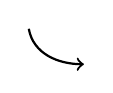
\begin{tikzpicture}
\draw [->,black,line width=0.8] (0,0) to [out=-80,in=180] (0.7,-0.45);
\end{tikzpicture}}
\put(118,-188){
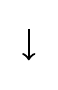
\begin{tikzpicture}
\draw [->,black,line width=0.8] (0,0) to (0,-0.4);
\end{tikzpicture}}

\put(212,-244){
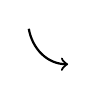
\begin{tikzpicture}
\draw [->,black,line width=0.8] (0,0) to [out=-80,in=180] (0.5,-0.45);
\end{tikzpicture}}
\put(206,-188){
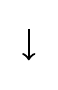
\begin{tikzpicture}
\draw [->,black,line width=0.8] (0,0) to (0,-0.4);
\end{tikzpicture}}
\end{picture}


%%%%% cele 3 lini
% culoare, grosime, plecare (cu minus),lungime

\begin{picture}(0,0)
\put(90,-260){\linie{gray}{3}{8.5}}
\end{picture}


\begin{picture}(0,0)
\put(185,-247){\linie{gray}{3}{8.5}}
\end{picture}

\begin{picture}(0,0)
\put(270,-232){\linie{gray}{3}{8.5}}
\end{picture}

\vspace{-11px}
%%%%%%%%%%%%%%%%%%%partea de sus

\hspace{-29px}\textit{\textbf{\fontsize{9pt}{0pt}\selectfont{\color{black}Goals:
}}}

%primul dreptughi
\begin{picture}(0,0)
\put(20,0)
{\dreptunghi{1.7cm}{0.6}{
\textbf{\fontsize{6pt}{0pt}\selectfont{\color{black}Articulate:\\
\textbullet who users are \\
\textbullet their key tasks
}}}}
\end{picture}


%dreptughiul 2
\begin{picture}(0,0)
\put(122,15)
{\dreptunghi{1.2cm}{0.6}{
\textbf{\fontsize{6pt}{0pt}\selectfont{\color{black}Brainstorm designs
}}}}
\end{picture}

%dreptughiul 3
\begin{picture}(0,0)
\put(212,30)
{\dreptunghi{1.2cm}{0.2}{
\textbf{\fontsize{6pt}{0pt}\selectfont{\color{black}Refined designs
}}}}
\end{picture}

%dreptughiul 4
\begin{picture}(0,0)
\put(285,42)
{\dreptunghi{1.1cm}{0.2}{
\textbf{\fontsize{6pt}{0pt}\selectfont{\color{gray}Completed designs
}}}}
\end{picture}


\vspace{30px}

%%%%%%%%%%%%%%%%%%%partea de mijloc

\hspace{-29px}\textit{\textbf{\fontsize{8.5pt}{0pt}\selectfont{\color{black}Methods:
}}}


%sageata 1
\vspace{20px}
 \begin{picture}(0,0)
 \put(-4,-12){\sageatainsus{5.5em}{7.4em}{4mm}{1.25cm}{0.4}{\fontsize{6pt}{1pt}\selectfont{\color{black}Task centered system \vspace{4px} design 
Participatory  \vspace{4px} design
User-centered design}}{-90}}
 \end{picture}
 
%sageata 2
 \begin{picture}(0,0)
\put(47,7){\sageatainsus{1.8em}{6.8em}{4.5mm}{0.9cm}{0.6}{\fontsize{6pt}{0pt}\selectfont{\color{black} Evaluate tasks}}{90}}
 \end{picture}


%sageata 3
\begin{picture}(0,0)
\put(90,18){\sageatainsus{5em}{7em}{5mm}{1.3cm}{0.4}{
\textbf{\fontsize{6pt}{0pt}\selectfont{\color{red} Psychology of everyday \vspace{4px}  things}}

\fontsize{6pt}{0pt}\selectfont{\color{black} User \vspace{4px} involvement}

\textbf{\fontsize{6pt}{0pt}\selectfont{\color{gray} Representation \& metaphors}}
}{-90}}
 \end{picture}
 
 
 %sageata 3 jos
\begin{picture}(0,0)
\put(90,-20){\sageatainsus{5em}{0em}{5mm}{1.2cm}{0.4}{
\textbf{\fontsize{6pt}{0pt}\selectfont{\color{black} low fidelity prototyping methods}}

}{-90}}
 \end{picture}
 
%sageata 4
\begin{picture}(0,0)
\put(137,50){\sageatainsus{4.5em}{7.4em}{5mm}{1.2cm}{0.4}{

\textit{\fontsize{6pt}{0pt}\selectfont{\color{black} Participatory \vspace{8px} interaction}}

\textit{\fontsize{6pt}{0pt}\selectfont{\color{black} Task scenario walk-through
}}

}{90}}
 \end{picture}

%sageata 5
\begin{picture}(0,0)
\put(185,60){\sageatainsus{4em}{7em}{5mm}{1cm}{0.4}{

\fontsize{6pt}{0pt}\selectfont{\color{gray}Graphical screen  \vspace{4px} design}

\fontsize{6pt}{0pt}\selectfont{\color{gray}Interface \vspace{4px} guidelines}

\fontsize{6pt}{0pt}\selectfont{\color{gray}Style  \vspace{4px} guides}

}{-90}}
 \end{picture}
 
 
 %sageata 5 jos
\begin{picture}(0,0)
\put(185,20){\sageatainsus{5em}{4em}{5mm}{1.2cm}{0.4}{
\textbf{\fontsize{6pt}{0pt}\selectfont{\color{black} high fidelity prototyping methods}}

}{-90}}
 \end{picture}

%sageata 6
\begin{picture}(0,0)
\put(228,88){\sageatainsus{4em}{7em}{5mm}{1cm}{0.4}{

\textit{\fontsize{6pt}{0pt}\selectfont{\color{black} Usability
 \vspace{8px} testing}}

\textit{\fontsize{6pt}{0pt}\selectfont{\color{gray} Heuristic evaluation}}
}{90}}
 \end{picture}

%sageata 7
\begin{picture}(0,0)
\put(296,103){\sageatainsus{2.5em}{7em}{3.6mm}{0.7cm}{0.4}{

\textit{\fontsize{6pt}{0pt}\selectfont{\color{gray}Field testing}}
}{90}}
 \end{picture}
 
 
 
 \vspace{-39px}
 %%%%%%%%%%%%%%%%%%%partea de jos

\hspace{-29px}\vspace{25px}\textit{\textbf{\fontsize{9pt}{0pt}\selectfont{\color{black}Products:
}}}

%dreptunghiul 1
\begin{picture}(0,0)
\put(20,27)
{\dreptunghi{1.4cm}{0.2}{
\textbf{\fontsize{6pt}{0pt}\selectfont{\color{black}User and task descriptions
}}}}
\end{picture}

%dreptunghiul 2
\begin{picture}(0,0)
\put(120,40)
{\dreptunghi{1.4cm}{0.2}{
\textbf{\fontsize{6pt}{0pt}\selectfont{\color{black}Throw-away paper prototypes
}}}}
\end{picture}

%dreptunghiul 3
\begin{picture}(0,0)
\put(205,56)
{\dreptunghi{1.2cm}{0.2}{
\textbf{\fontsize{6pt}{0pt}\selectfont{\color{black}Testable prototypes
}}}}
\end{picture}

%dreptunghiul 4
\begin{picture}(0,0)
\put(280,60)
{\dreptunghi{1.4cm}{0.2}{
\textbf{\fontsize{6pt}{0pt}\selectfont{\color{gray}Alpha/beta systems or complete specification
}}}}
\end{picture}
\end{frame}



{\setbeamercolor{background canvas}{bg=background}
\setbeamercolor{normal text}{fg=Blue}
\usebeamercolor[fg]{normal text}
\begin{frame}
	{*Bibliography}{\textcolor{red}{\rule{12cm}{1.2pt}}}

        \begin{itemize}
        	\item[{$\bullet$}] Saul Greenberg, \textbf{Designing and building visual interfaces. Design of Everyday Things}, University of Calgary, Canada

        	\url{http://pages.cpsc.ucalgary.ca/~saul/481/}
        	\newline
        	 
        	\item[{$\bullet$}] Keith Andrews, \textbf{Human Computer Interaction, Chapter 2. The Psychology of Usable Things}, TU Graz, Austria

        	\url{https://courses.isds.tugraz.at/hci/hci.pdf}                			\newline
     	\end{itemize}
\end{frame}



\end{document}